\begin{figure}
	\centering
	\begin{subfigure}{0.48\columnwidth}
		\centering
		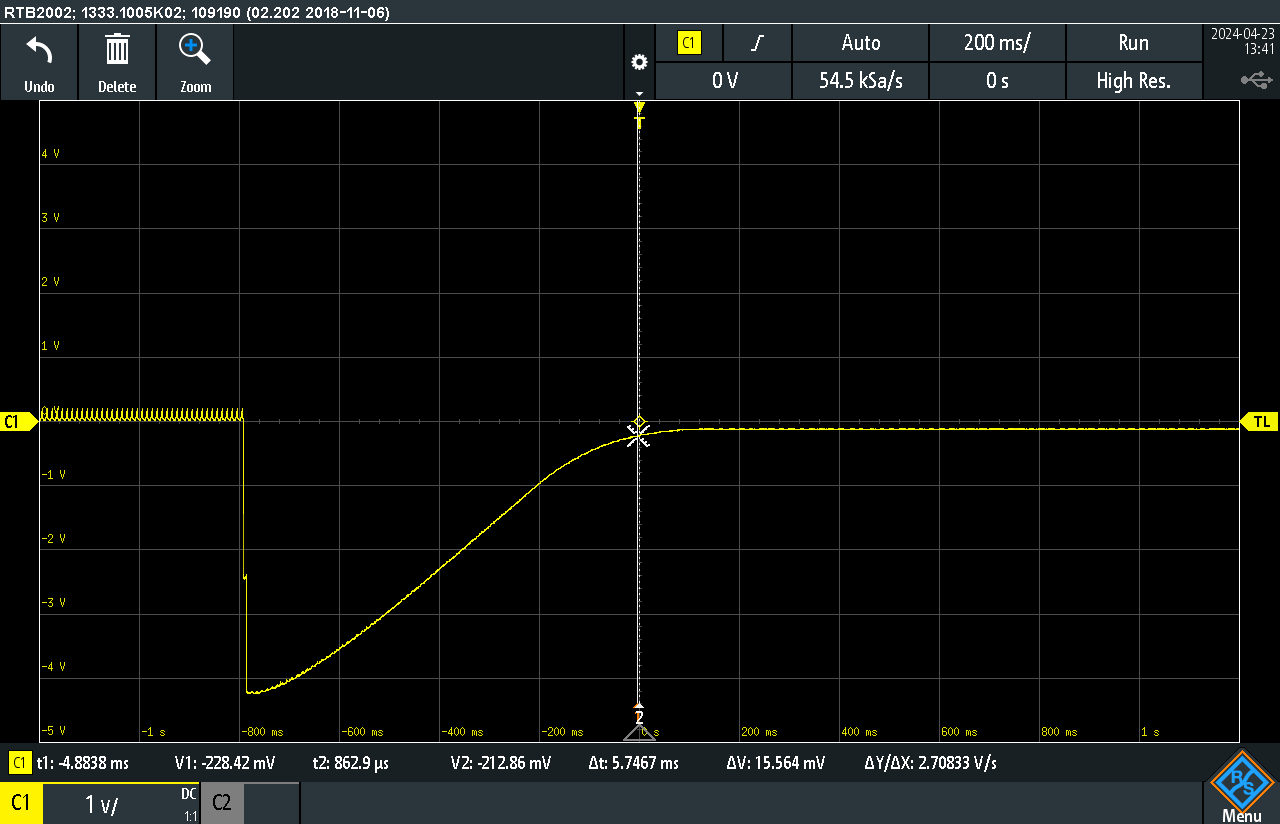
\includegraphics[width=0.8\linewidth]{src/figures/oscilloscope-raw/p60-d0.png}
		\subcaption{P=60, D=0}\label{fig:oscilloscope-raw-p60-d0}
	\end{subfigure}
	\begin{subfigure}{0.48\columnwidth}
		\centering
		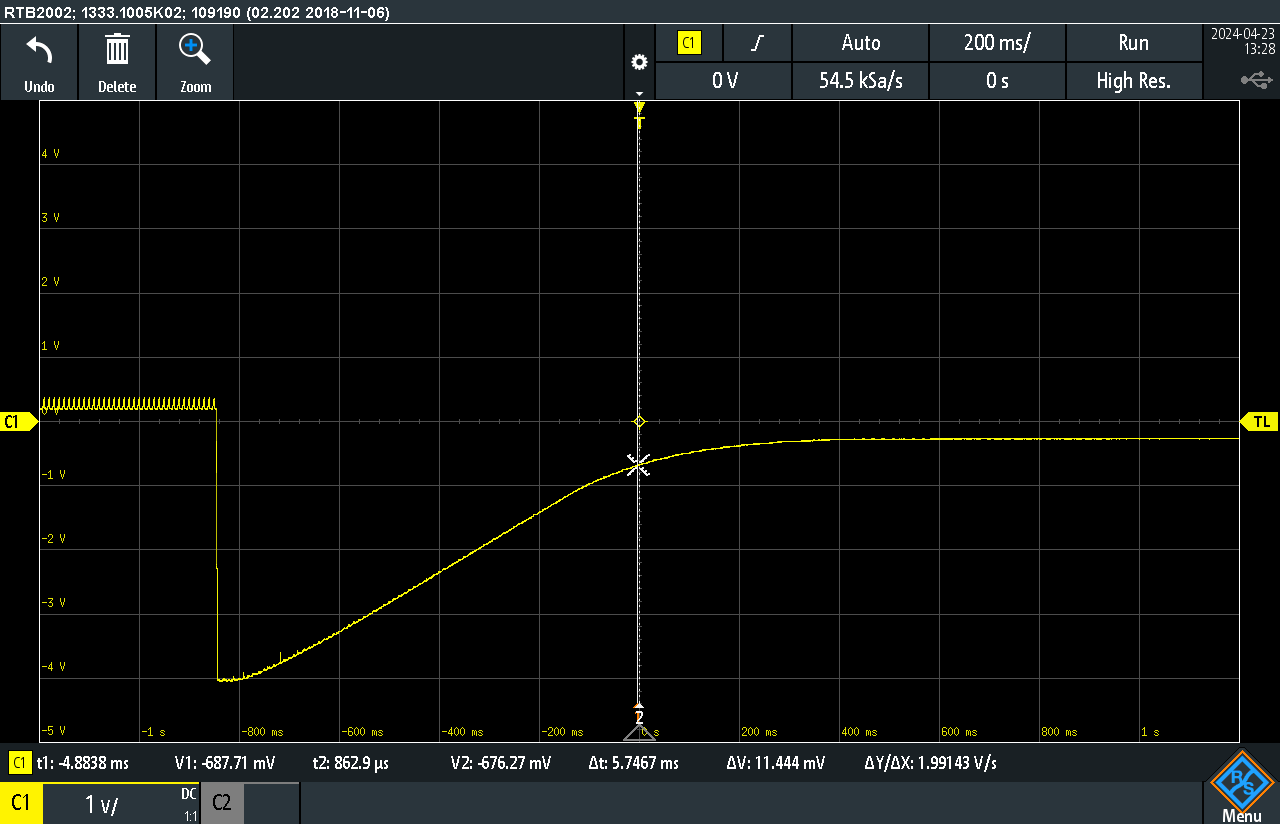
\includegraphics[width=0.8\linewidth]{src/figures/oscilloscope-raw/p60-d60.png}
		\subcaption{P=60, D=60}\label{fig:oscilloscope-raw-p60-d60}
	\end{subfigure}
	\begin{subfigure}{0.48\columnwidth}
		\centering
		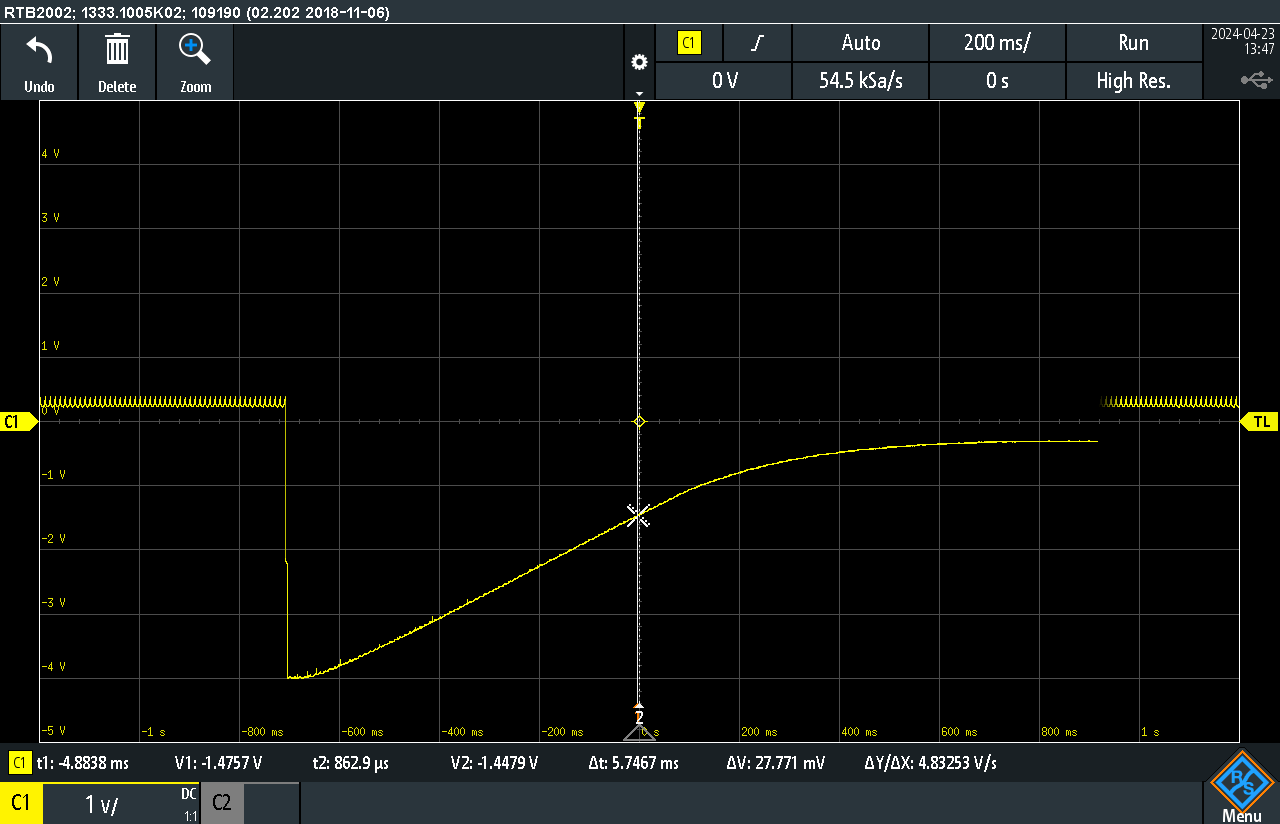
\includegraphics[width=0.8\linewidth]{src/figures/oscilloscope-raw/p60-d80.png}
		\subcaption{P=60, D=80}\label{fig:oscilloscope-raw-p60-d80}
	\end{subfigure}
	\begin{subfigure}{0.48\columnwidth}
		\centering
		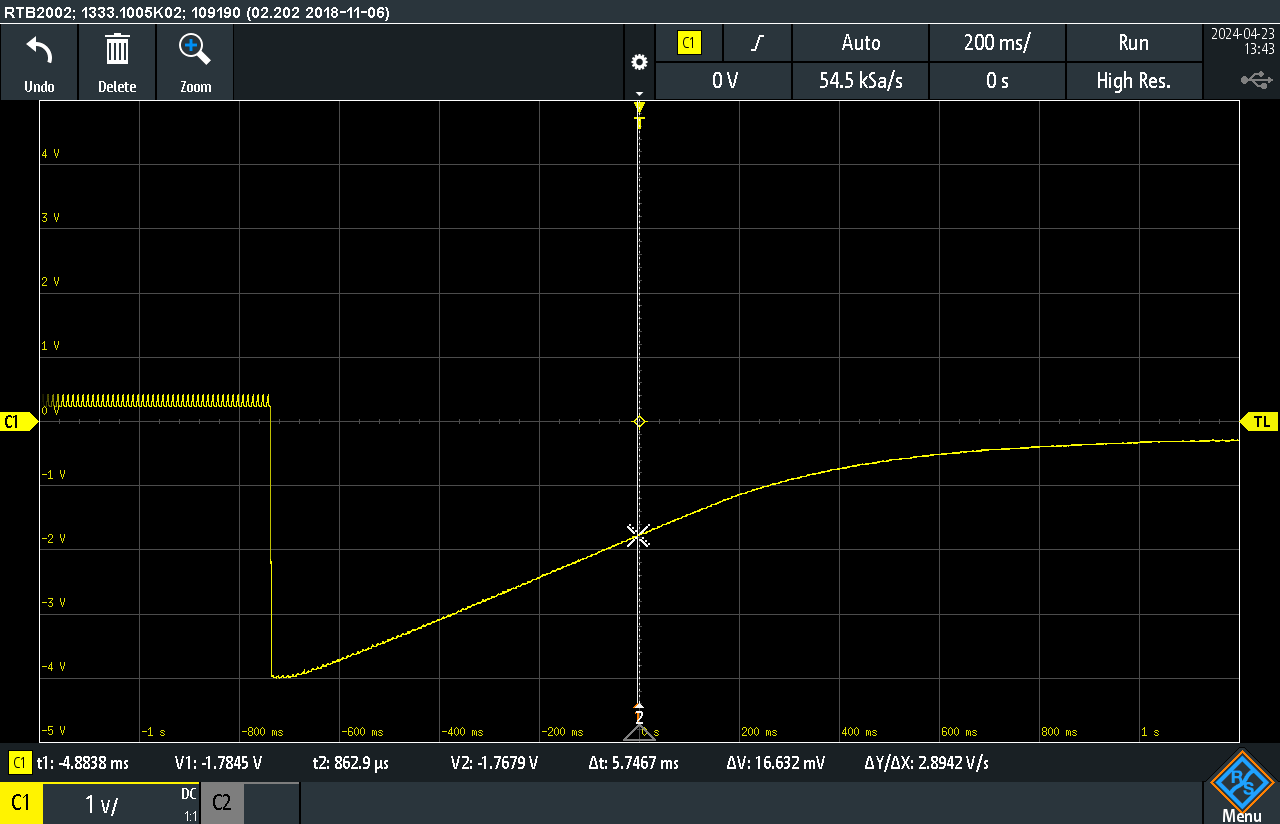
\includegraphics[width=0.8\linewidth]{src/figures/oscilloscope-raw/p60-d100.png}
		\subcaption{P=60, D=100}\label{fig:oscilloscope-raw-p60-d100}
	\end{subfigure}
\end{figure}

\begin{figure}
	\setcounter{figure}{-1}
	\centering
	\begin{subfigure}{0.48\columnwidth}
		\setcounter{subfigure}{4}
		\centering
		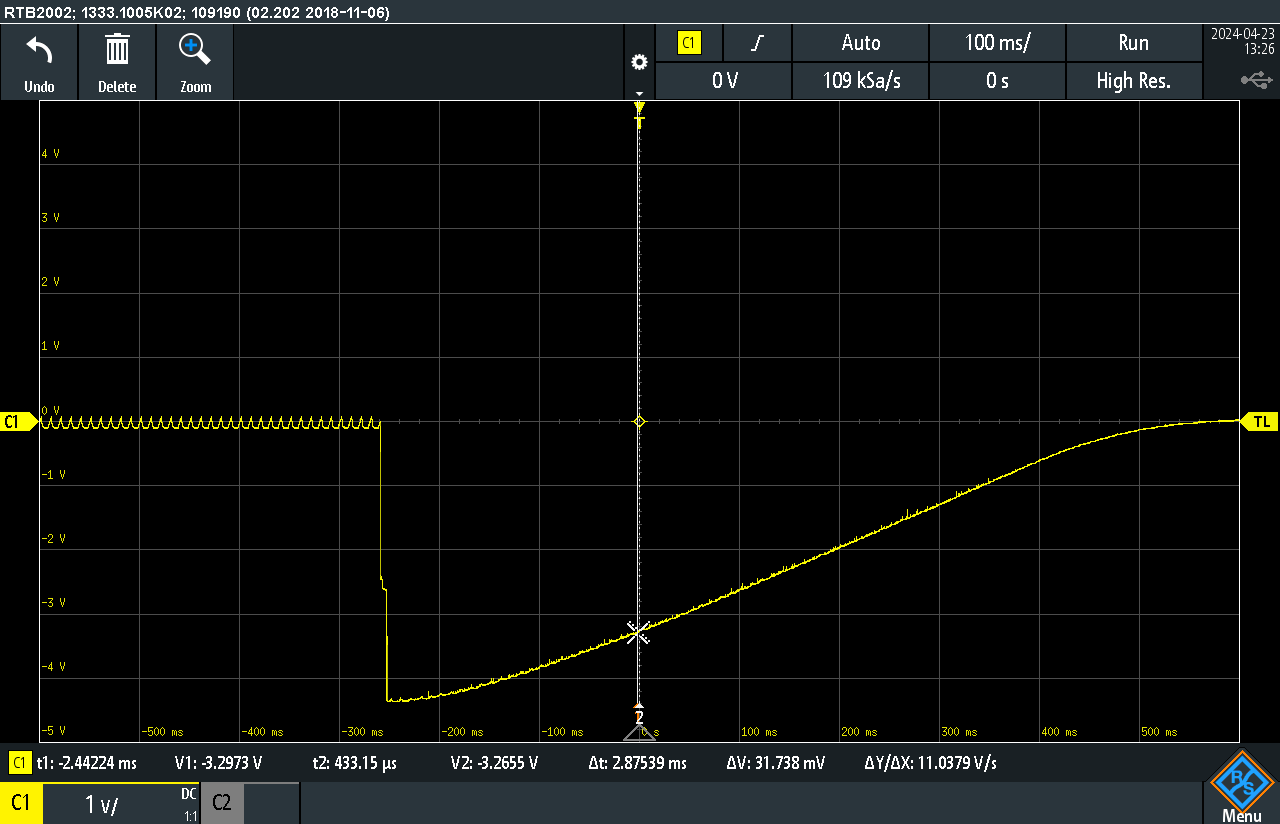
\includegraphics[width=0.8\linewidth]{src/figures/oscilloscope-raw/p80-d0.png}
		\subcaption{P=80, D=0}\label{fig:oscilloscope-raw-p80-d0}
	\end{subfigure}
	\begin{subfigure}{0.48\columnwidth}
		\centering
		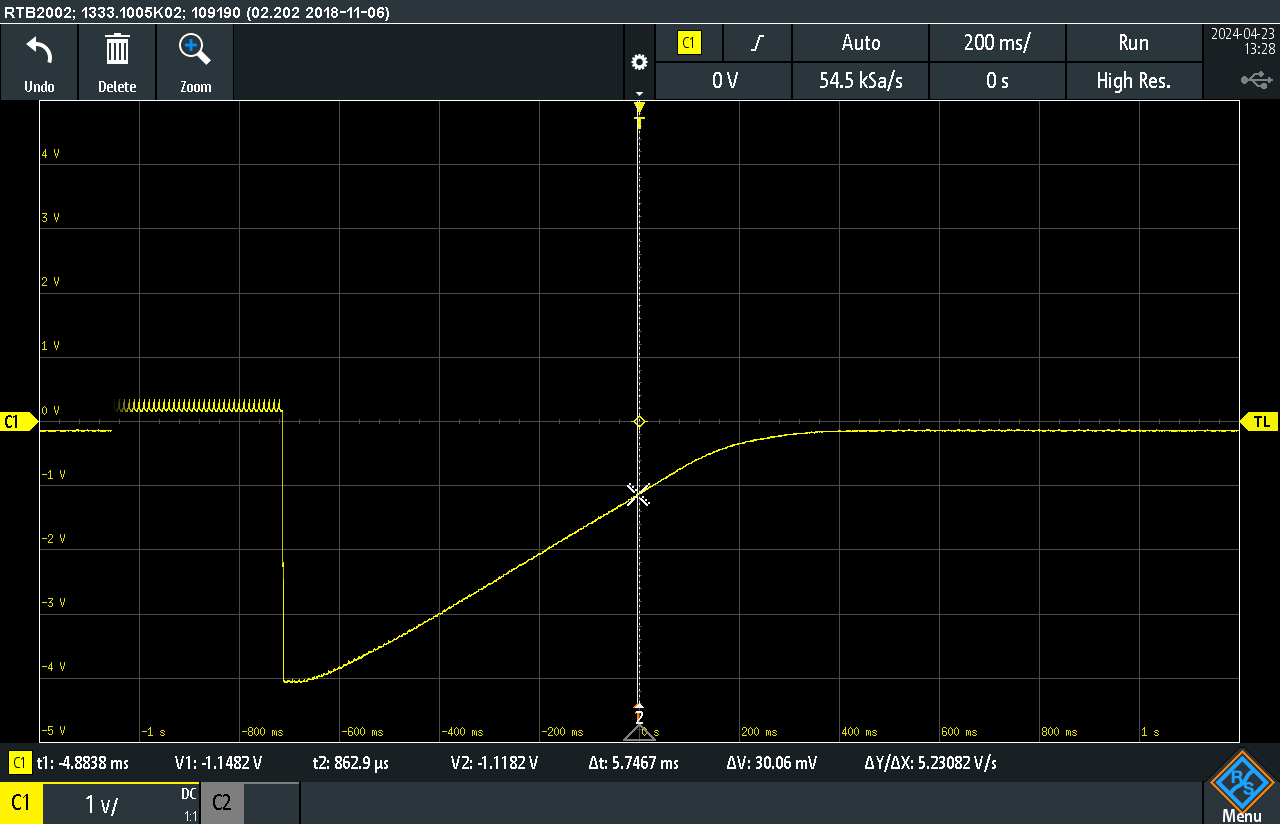
\includegraphics[width=0.8\linewidth]{src/figures/oscilloscope-raw/p80-d60.png}
		\subcaption{P=80, D=60}\label{fig:oscilloscope-raw-p80-d60}
	\end{subfigure}
	\begin{subfigure}{0.48\columnwidth}
		\centering
		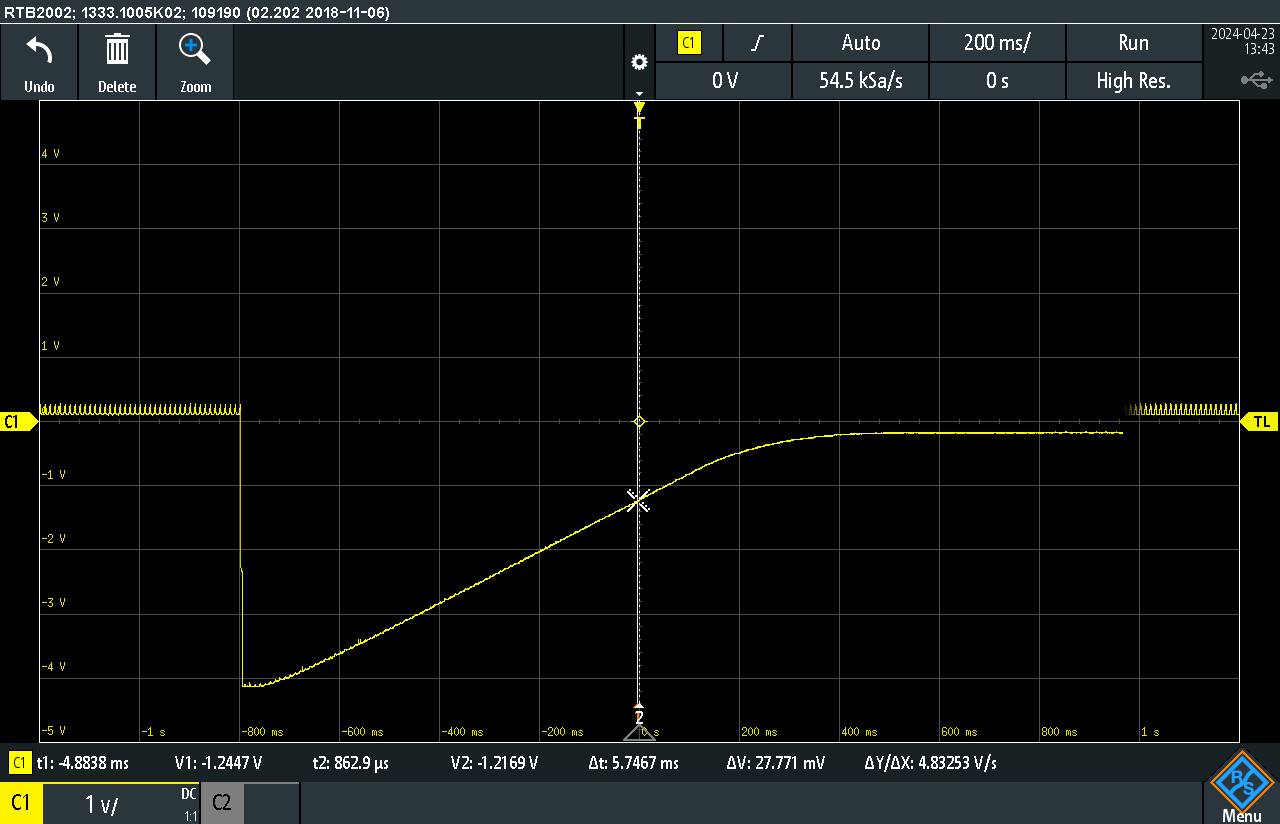
\includegraphics[width=0.8\linewidth]{src/figures/oscilloscope-raw/p80-d80.png}
		\subcaption{P=80, D=80}\label{fig:oscilloscope-raw-p80-d80}
	\end{subfigure}
	\begin{subfigure}{0.48\columnwidth}
		\centering
		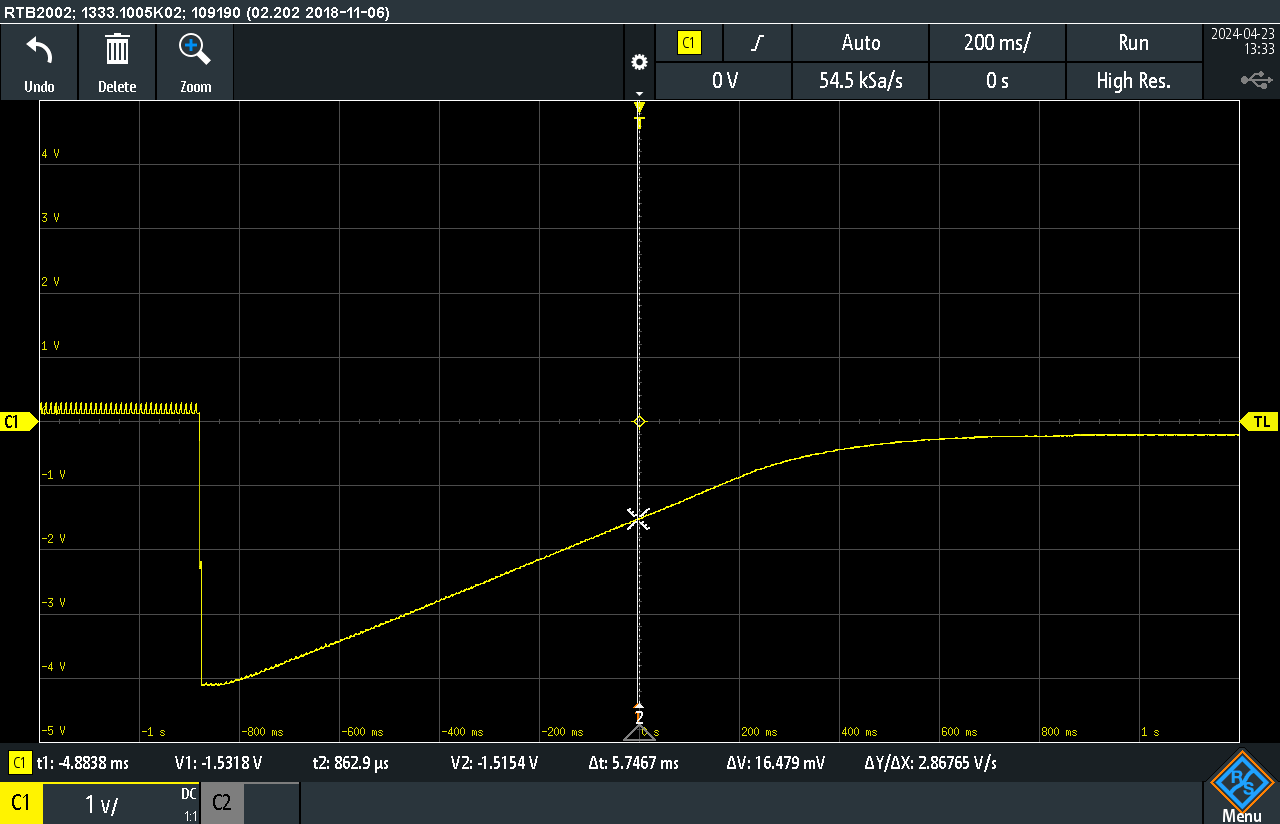
\includegraphics[width=0.8\linewidth]{src/figures/oscilloscope-raw/p80-d100.png}
		\subcaption{P=80, D=100}\label{fig:oscilloscope-raw-p80-d100}
	\end{subfigure}

\end{figure}

\begin{figure}
	\setcounter{figure}{-1}
	\centering
	\begin{subfigure}{0.48\columnwidth}
		\setcounter{subfigure}{4}
		\centering
		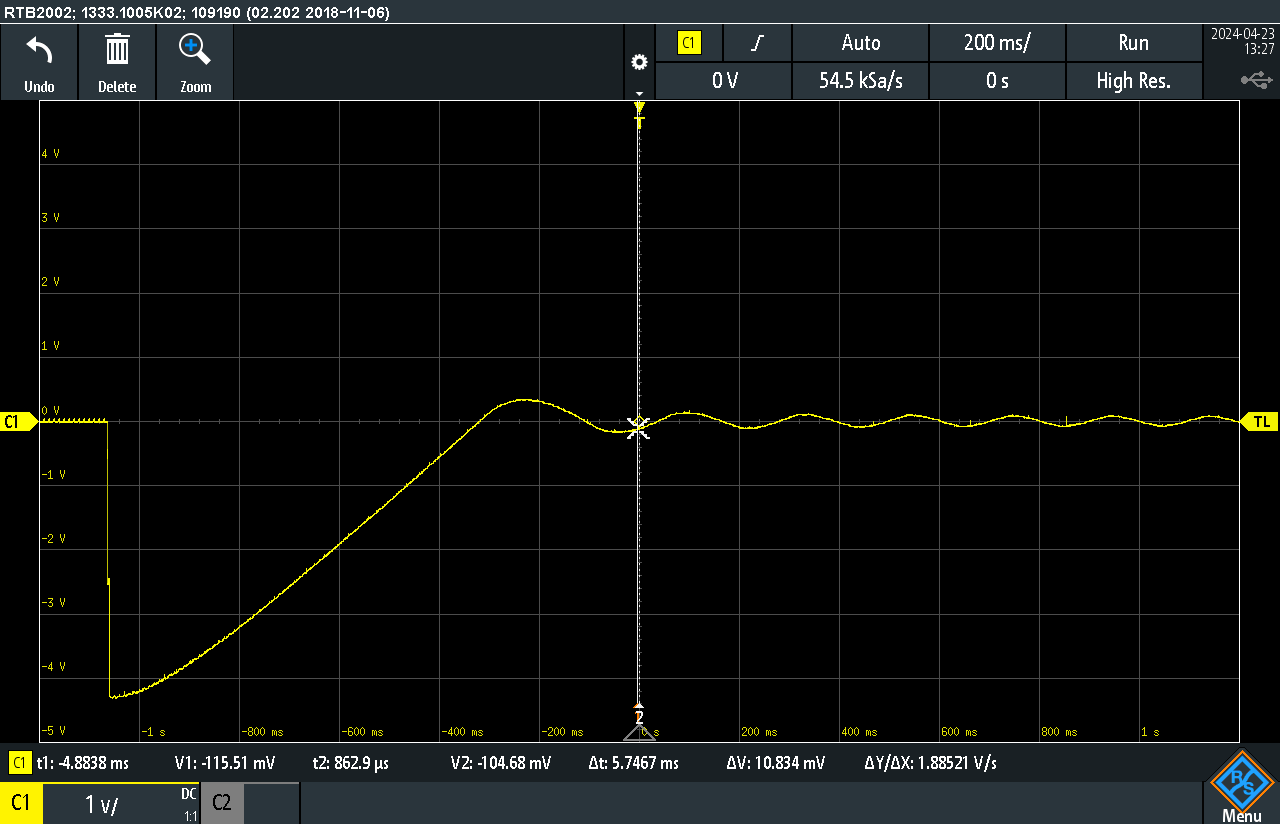
\includegraphics[width=0.8\linewidth]{src/figures/oscilloscope-raw/p100-d0.png}
		\subcaption{P=100, D=0}\label{fig:oscilloscope-raw-p100-d0}
	\end{subfigure}
	\begin{subfigure}{0.48\columnwidth}
		\centering
		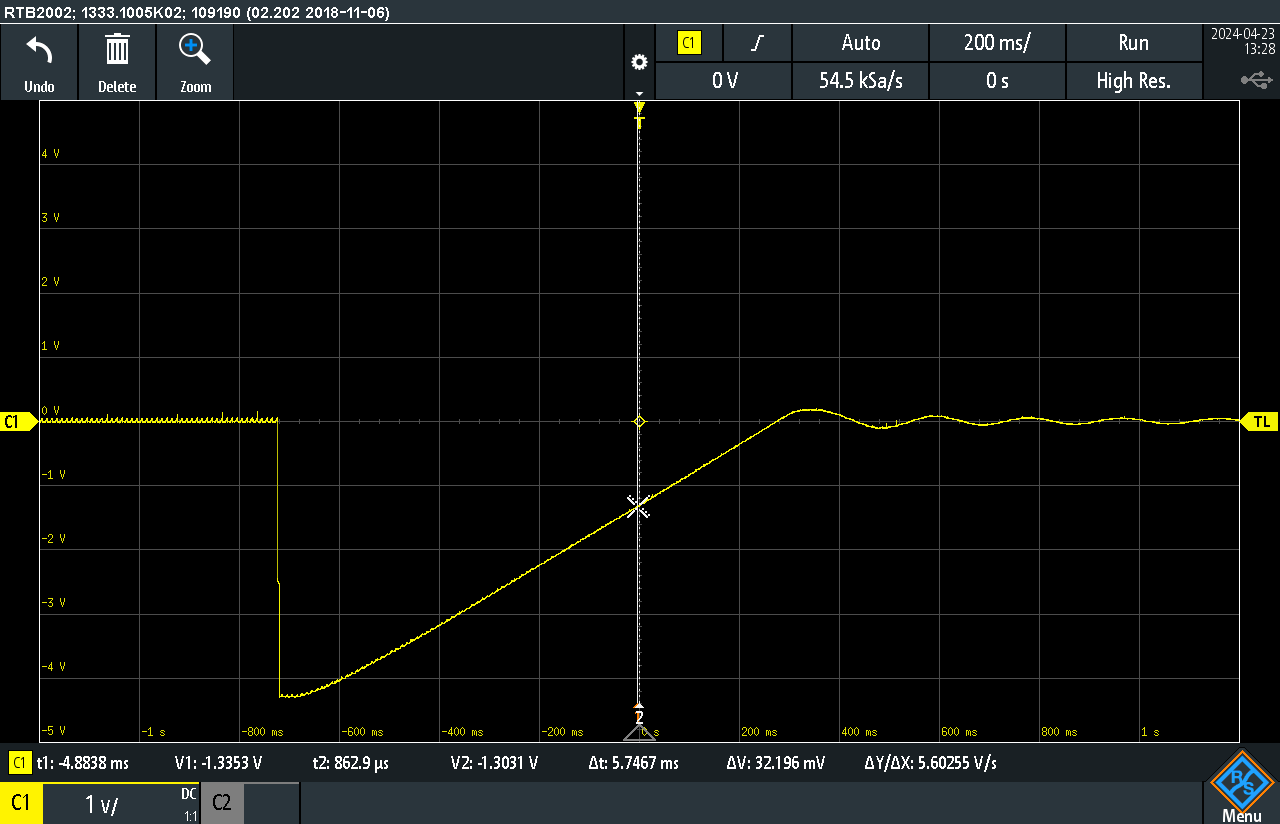
\includegraphics[width=0.8\linewidth]{src/figures/oscilloscope-raw/p100-d60.png}
		\subcaption{P=100, D=60}\label{fig:oscilloscope-raw-p100-d60}
	\end{subfigure}
	\begin{subfigure}{0.48\columnwidth}
		\centering
		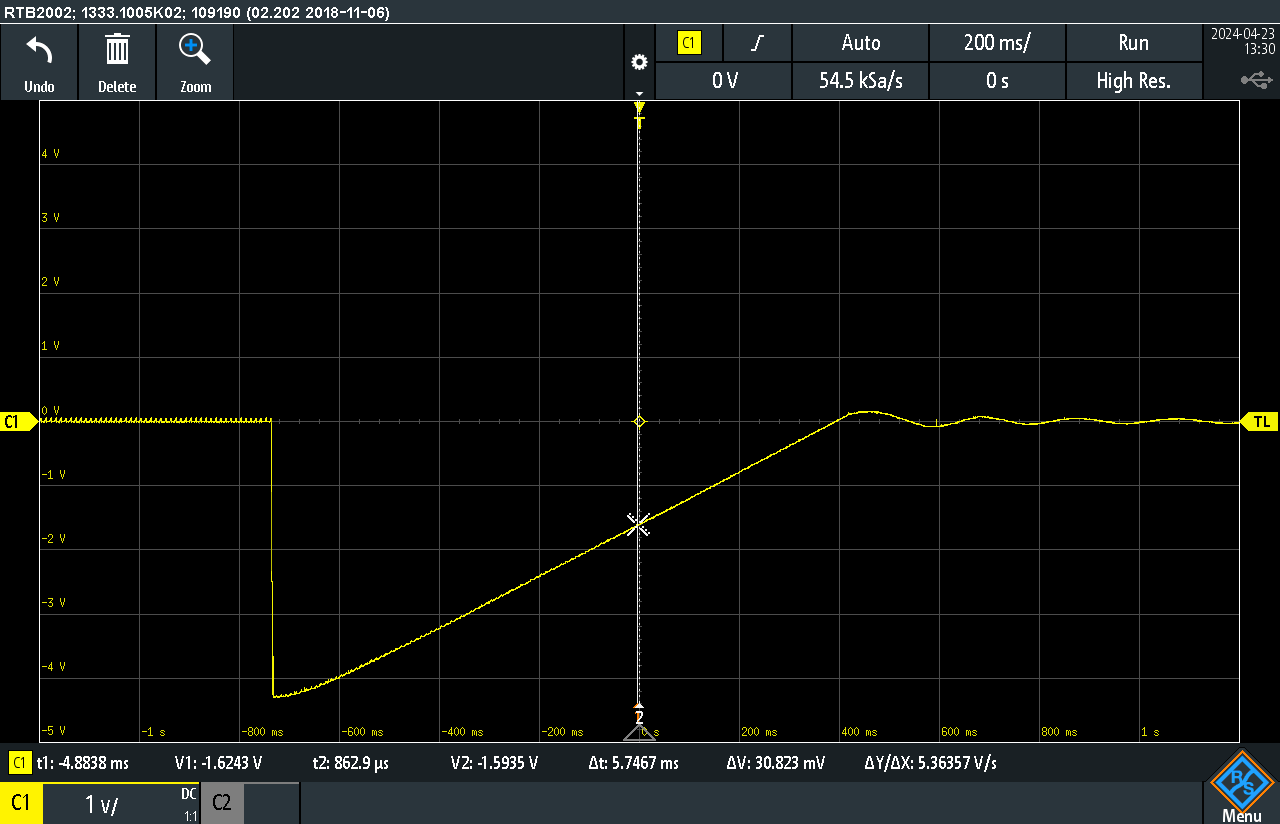
\includegraphics[width=0.8\linewidth]{src/figures/oscilloscope-raw/p100-d80.png}
		\subcaption{P=100, D=80}\label{fig:oscilloscope-raw-p100-d80}
	\end{subfigure}
	\begin{subfigure}{0.48\columnwidth}
		\centering
		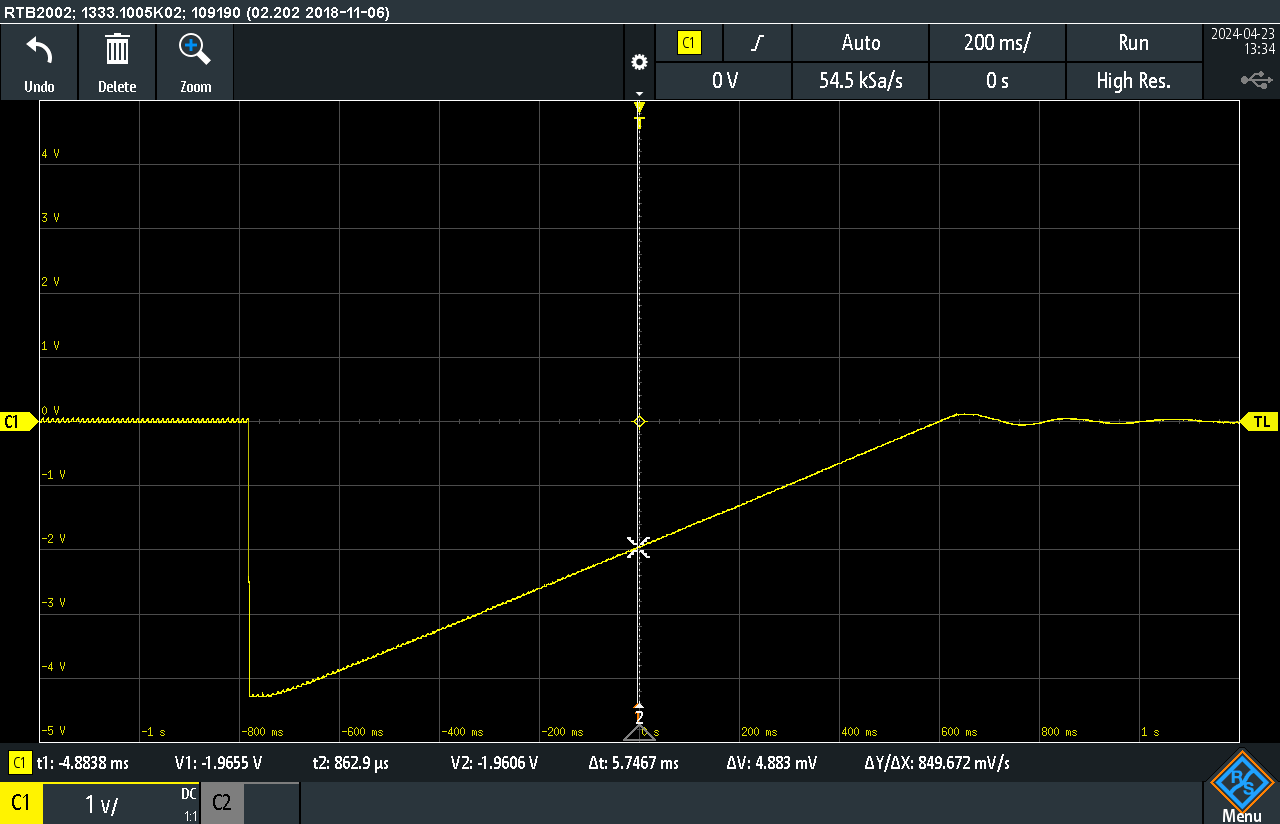
\includegraphics[width=0.8\linewidth]{src/figures/oscilloscope-raw/p100-d100.png}
		\subcaption{P=100, D=100}\label{fig:oscilloscope-raw-p100-d100}
	\end{subfigure}

	\caption{各制御パラメータにおけるオシロスコープの波形}\label{fig:oscilloscope-raw}
\end{figure}
